\section{Introduction}
The main objective of this work is to investigate new strategies for
two-sided bidiagonal factorization,
which is widely used to
transform a full matrix into bidiagonal form using orthogonal transformations.
A matrix bidiagonalization is required as a precursor to computing the
singular value decomposition (SVD).
The SVD of an $m\times n$ matrix $A$ is given by:
$A = U \Sigma V^T$ or ($A = U \Sigma V^H$ if A is complex) where
$U$ and $V$ are orthogonal (unitary) and $\Sigma$ is an $m\times n$
matrix with real diagonal elements, $\sigma_i$ , commonly ordered such
that: $\sigma_1 \ge \sigma_2 \ge \dots \ge \sigma_{min(m,n)} \ge 0.$
The $\sigma_i$ are known as the singular values of $A$
and the first $\min(m, n)$ columns
of $U$ and $V$ are the left and right singular vectors of $A$, respectively.

For a given $m\times n$ matrix $A$,
the traditional approach, for computing the singular
values and optionally the singular vectors,
consists of the following steps:
\begin{enumerate}
\item Reduction of the matrix $A$ to bidiagonal form: $A =
  U_1BV^T_1$ if $A$ is real ($A = U_1BV^H_1$ if $A$ is complex), where
  $U_1$ and $V_1$ are orthogonal (unitary if $A$ is complex), and $B$ is
  real and upper bidiagonal when $m \ge n$ or lower bidiagonal when $m < n$,
  so that $B$ is nonzero on only the main diagonal and either the first
  superdiagonal (if $m \ge n$) or the first subdiagonal (if $m < n$).

\item The SVD computation of the bidiagonal matrix $B$: $B = U_2 \Sigma
  V_2^T$, where $U_2$ and $V_2$ are orthogonal, and $\Sigma$ is
  diagonal with entries consisting of the singular values of $A$.
\item If required, the singular vectors of $A$ are computed as
  $U = U_1U_2$ and $V = V_1 V_2$.
\end{enumerate}

The SVD decomposition algorithm described above was introduced in
1965 by Golub and Kahan~\cite{golub1965calculating}.
While the last two steps have been considerably optimized
for modern architectures,
the first step---%
the reduction to bidiagonal form---%
remains limited by
memory-bound operations.
In fact, in the algorithm proposed by Golub,
the reduction to bidiagonal form is achieved by applying a QR step to
the first column, followed by a LQ step to the first row, then a QR
step to the second column, and so on. Since this algorithm processes
one column (or row) at a time using Householder transformations,
it is limited to Level-2 BLAS kernels (and is hence memory-bound).

In 1989, to improve the bidiagonalization step,
Dongarra, Sorensen, and Hammarling~\cite{dongarra1989block}
proposed a new variant which has the advantage of exploiting
Level-3 BLAS operations.
Instead of applying the householder transformations to
one column at a time,
their algorithm uses a aggregated householder transformations
strategy~\cite{bischof1987wy} to process a few columns at a time,
giving us the opportunity to use compute-intensive Level-3 BLAS kernels.
This modification to the bidiagonalization algorithm helps
to reformulate approximately 50\% of the process as Level-3 BLAS operations
as reported by Gro{\ss}er and Lang in~\cite{grosser1999efficient}.

To address the remaining 50\% of Level-2 BLAS operations in the
algorithm, in 1999, Gro{\ss}er and Lang introduced a two-staged
approach.
As illustrated in Figure~\ref{fig:two_stage},
the first stage consists of reducing the full matrix into a
band bidiagonal form (Figure~\ref{fig:SVD_band_bidiag}) using only
compute-intensive kernels,
followed by a second stage to reduce the band
matrix to a bidiagonal form (Figure~\ref{fig:SVD_bidiag}) with
memory-bound kernels.
Since the first stage is a compute-intensive
algorithm and represents the dominant part of the process,
it significantly increases the overall performance of the
bidiagonalization process.
This two-stage algorithm may introduce extra flops
but as reported by Azzam~et~al\@.~\cite{haidar2013improved},
it is still efficient in terms of time to solution.

In this work, we consider the two-stage bidiagonalization algorithm
with a special focus on the first stage.
We compare various design options making use of tile algorithms and
the task-based programming model.
As a result,
we propose a prototype based on the OpenMP 4.0 runtime system which is
competitive with state-of-the-art implementations.
The remainder of this paper is organized as follows.
In section~\ref{sec:tile} we explain the background to tiled algorithms.
Then, in section~\ref{sec:band} we discuss and analyze
different strategies for implementing the
reduction from a full matrix to band bidiagonal form,
followed by performance analyses and a discussion of
the potential performance improvement.
Section~\ref{sec:bidiag} investigates different solutions
for transforming the band bidiagonal matrix
to bidiagonal form before providing some concluding
remarks in Section~\ref{sec:conclusion}.

\begin{figure}[h!]
  \begin{subfigure}[t]{0.3 \textwidth}
    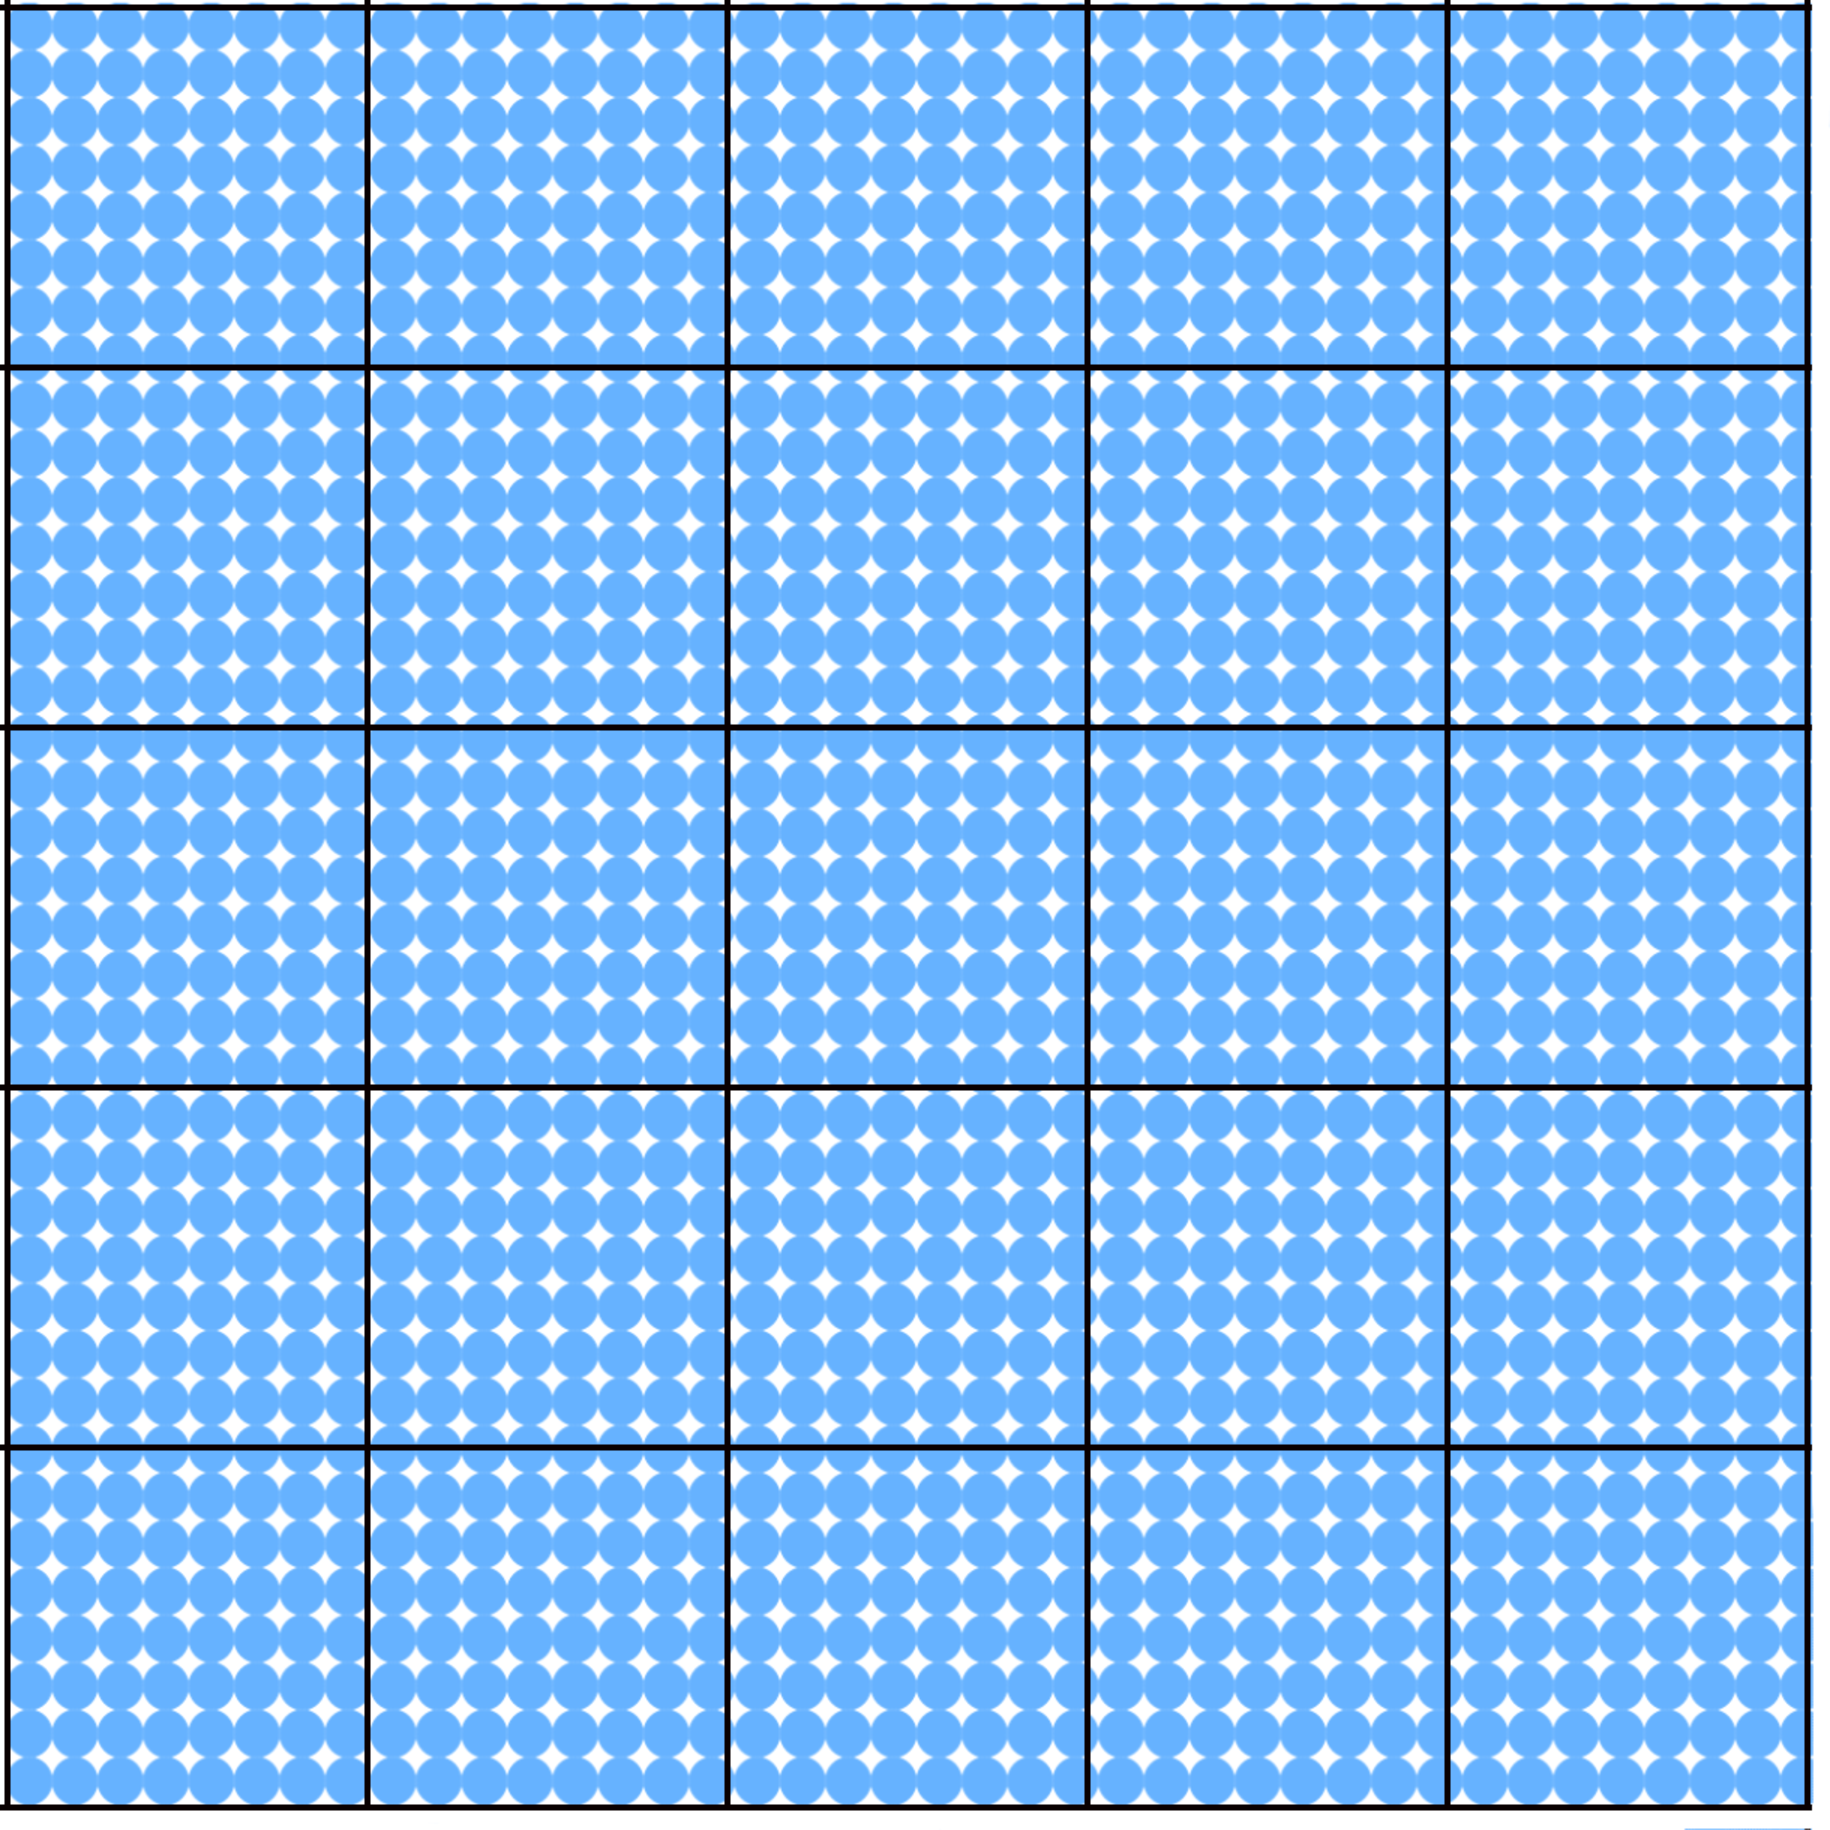
\includegraphics[width=3.5cm, height=3.5cm]{fig/SVD_1_grid}
    \caption{\label{fig:SVD_initial}Full $5\times 5$ tile matrix.}
  \end{subfigure}
  \hfill
  \begin{subfigure}[t]{0.3 \textwidth}
    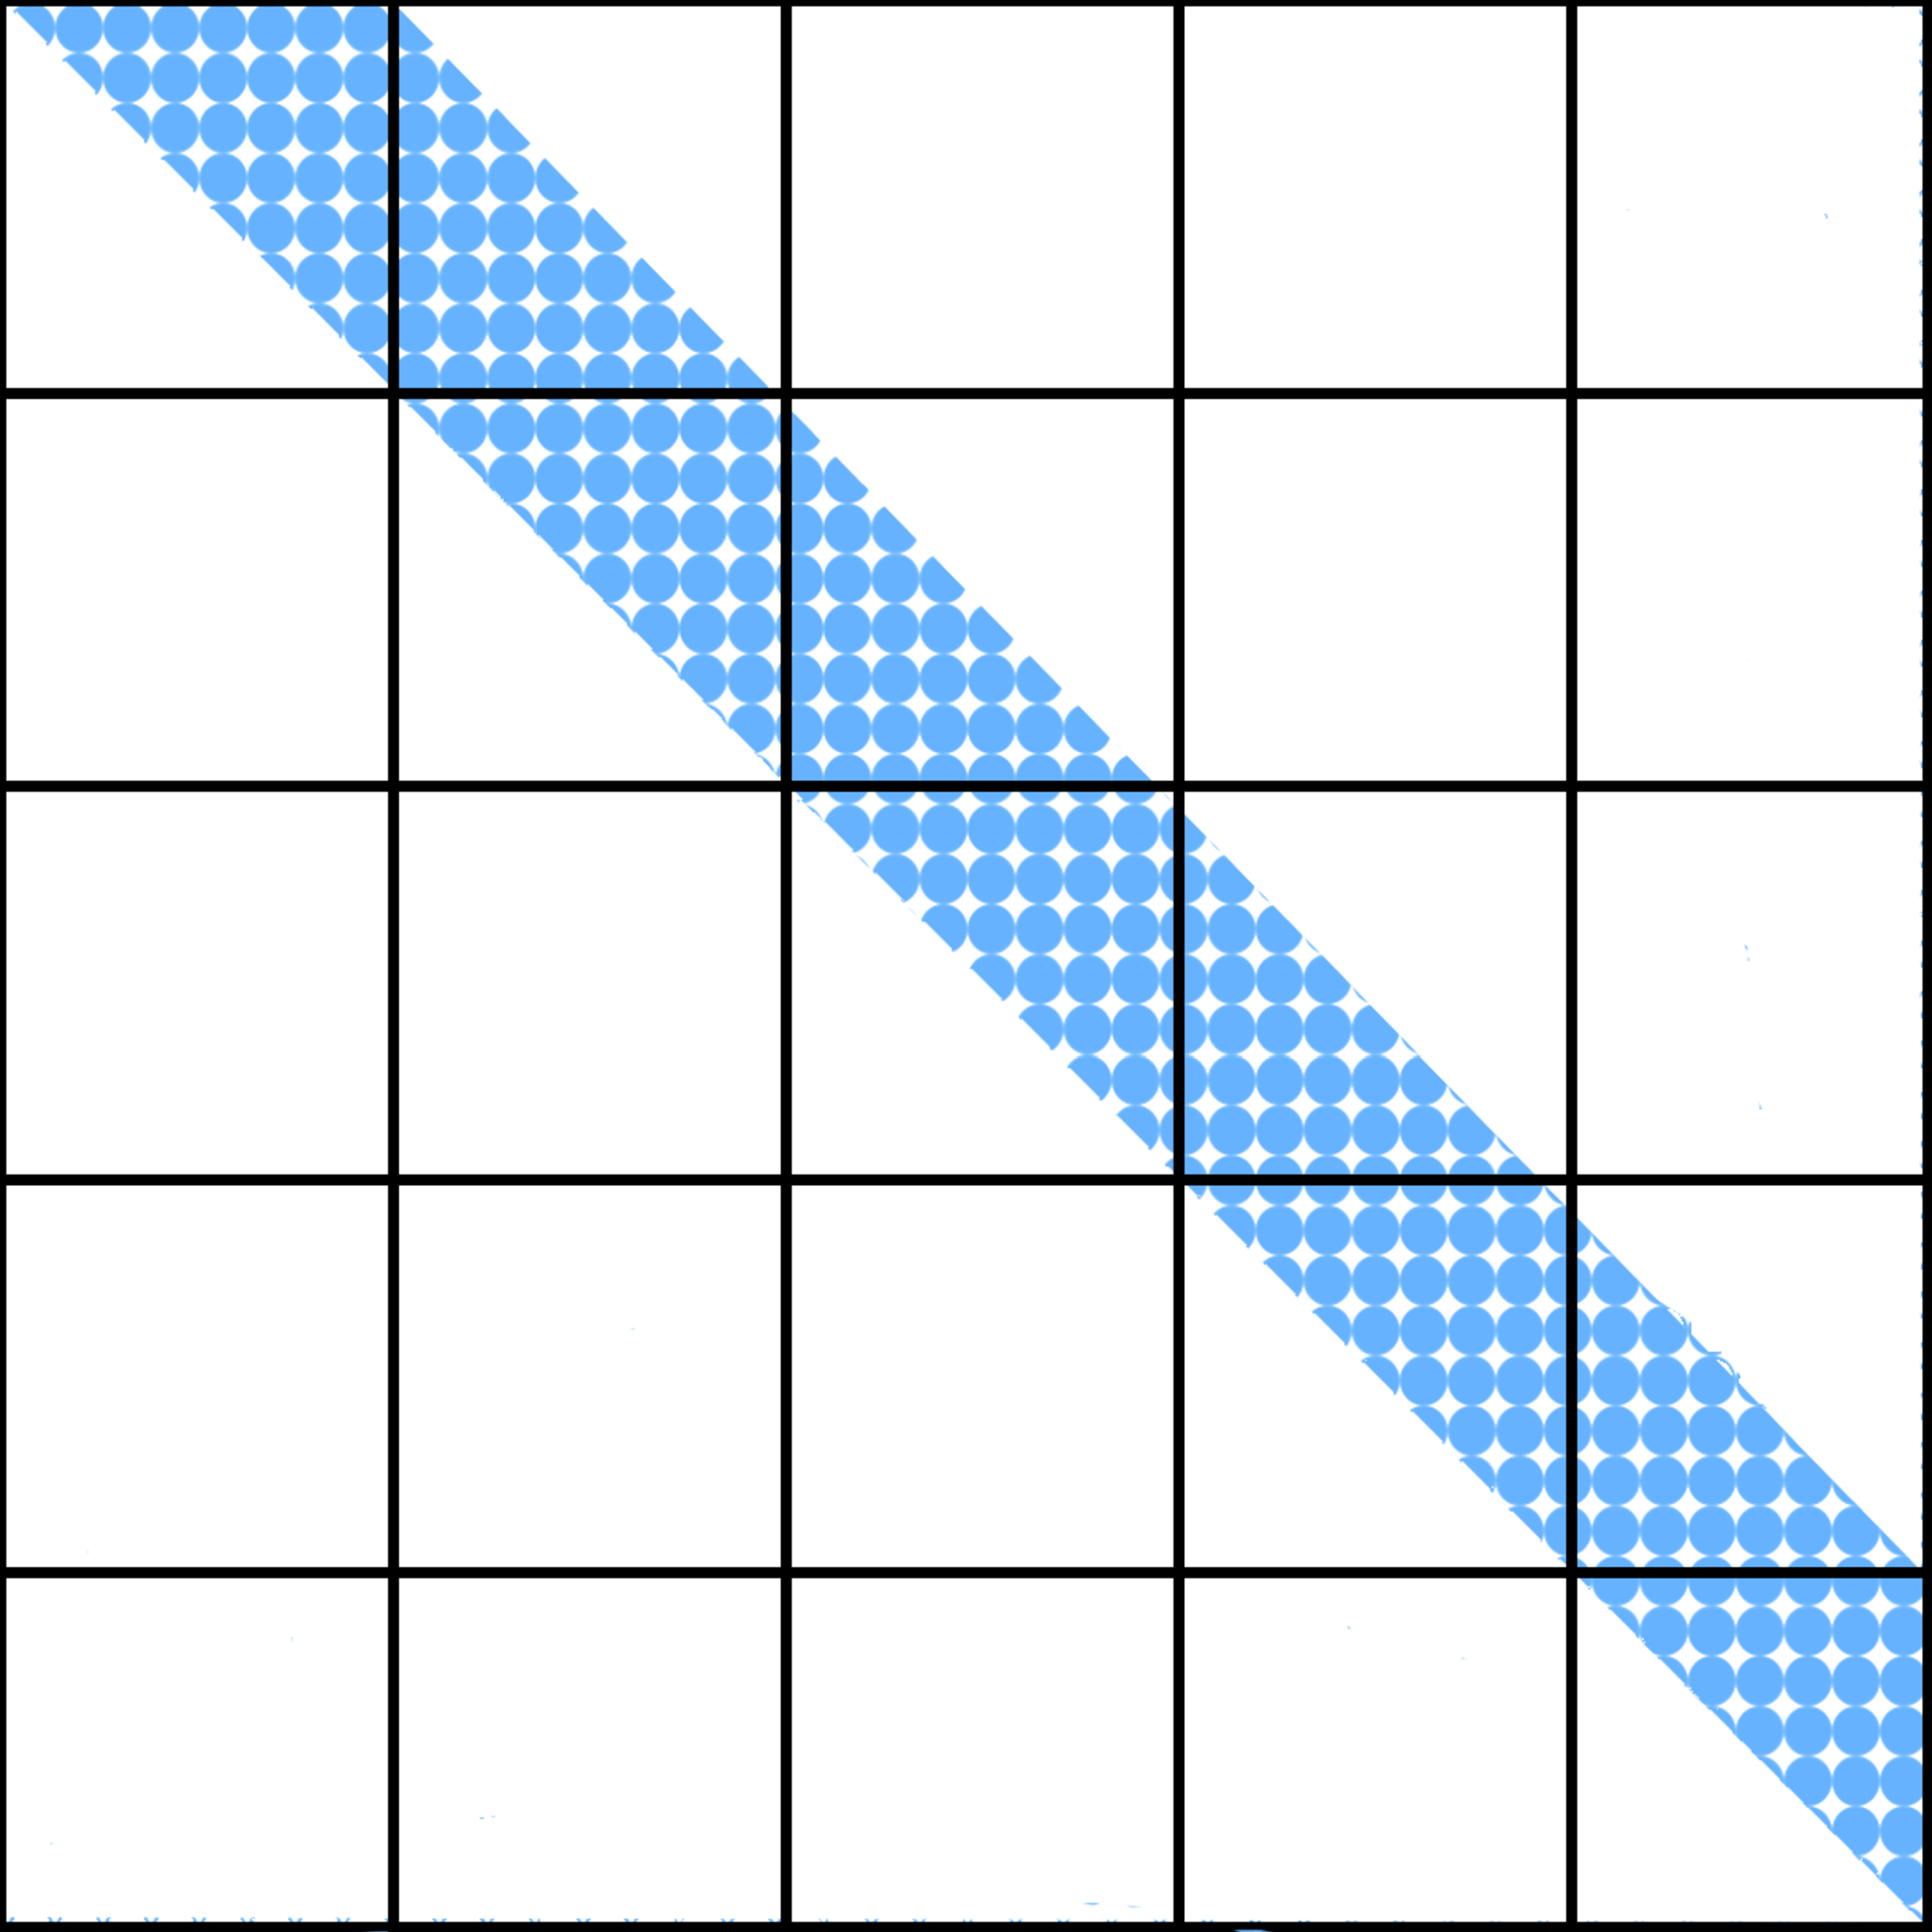
\includegraphics[width=3.5cm, height=3.5cm]{fig/SVD_band_bidiag}
    \caption{\label{fig:SVD_band_bidiag}
     Band bidiagonal form.}
  \end{subfigure}
  \hfill
    \begin{subfigure}[t]{0.3 \textwidth}
    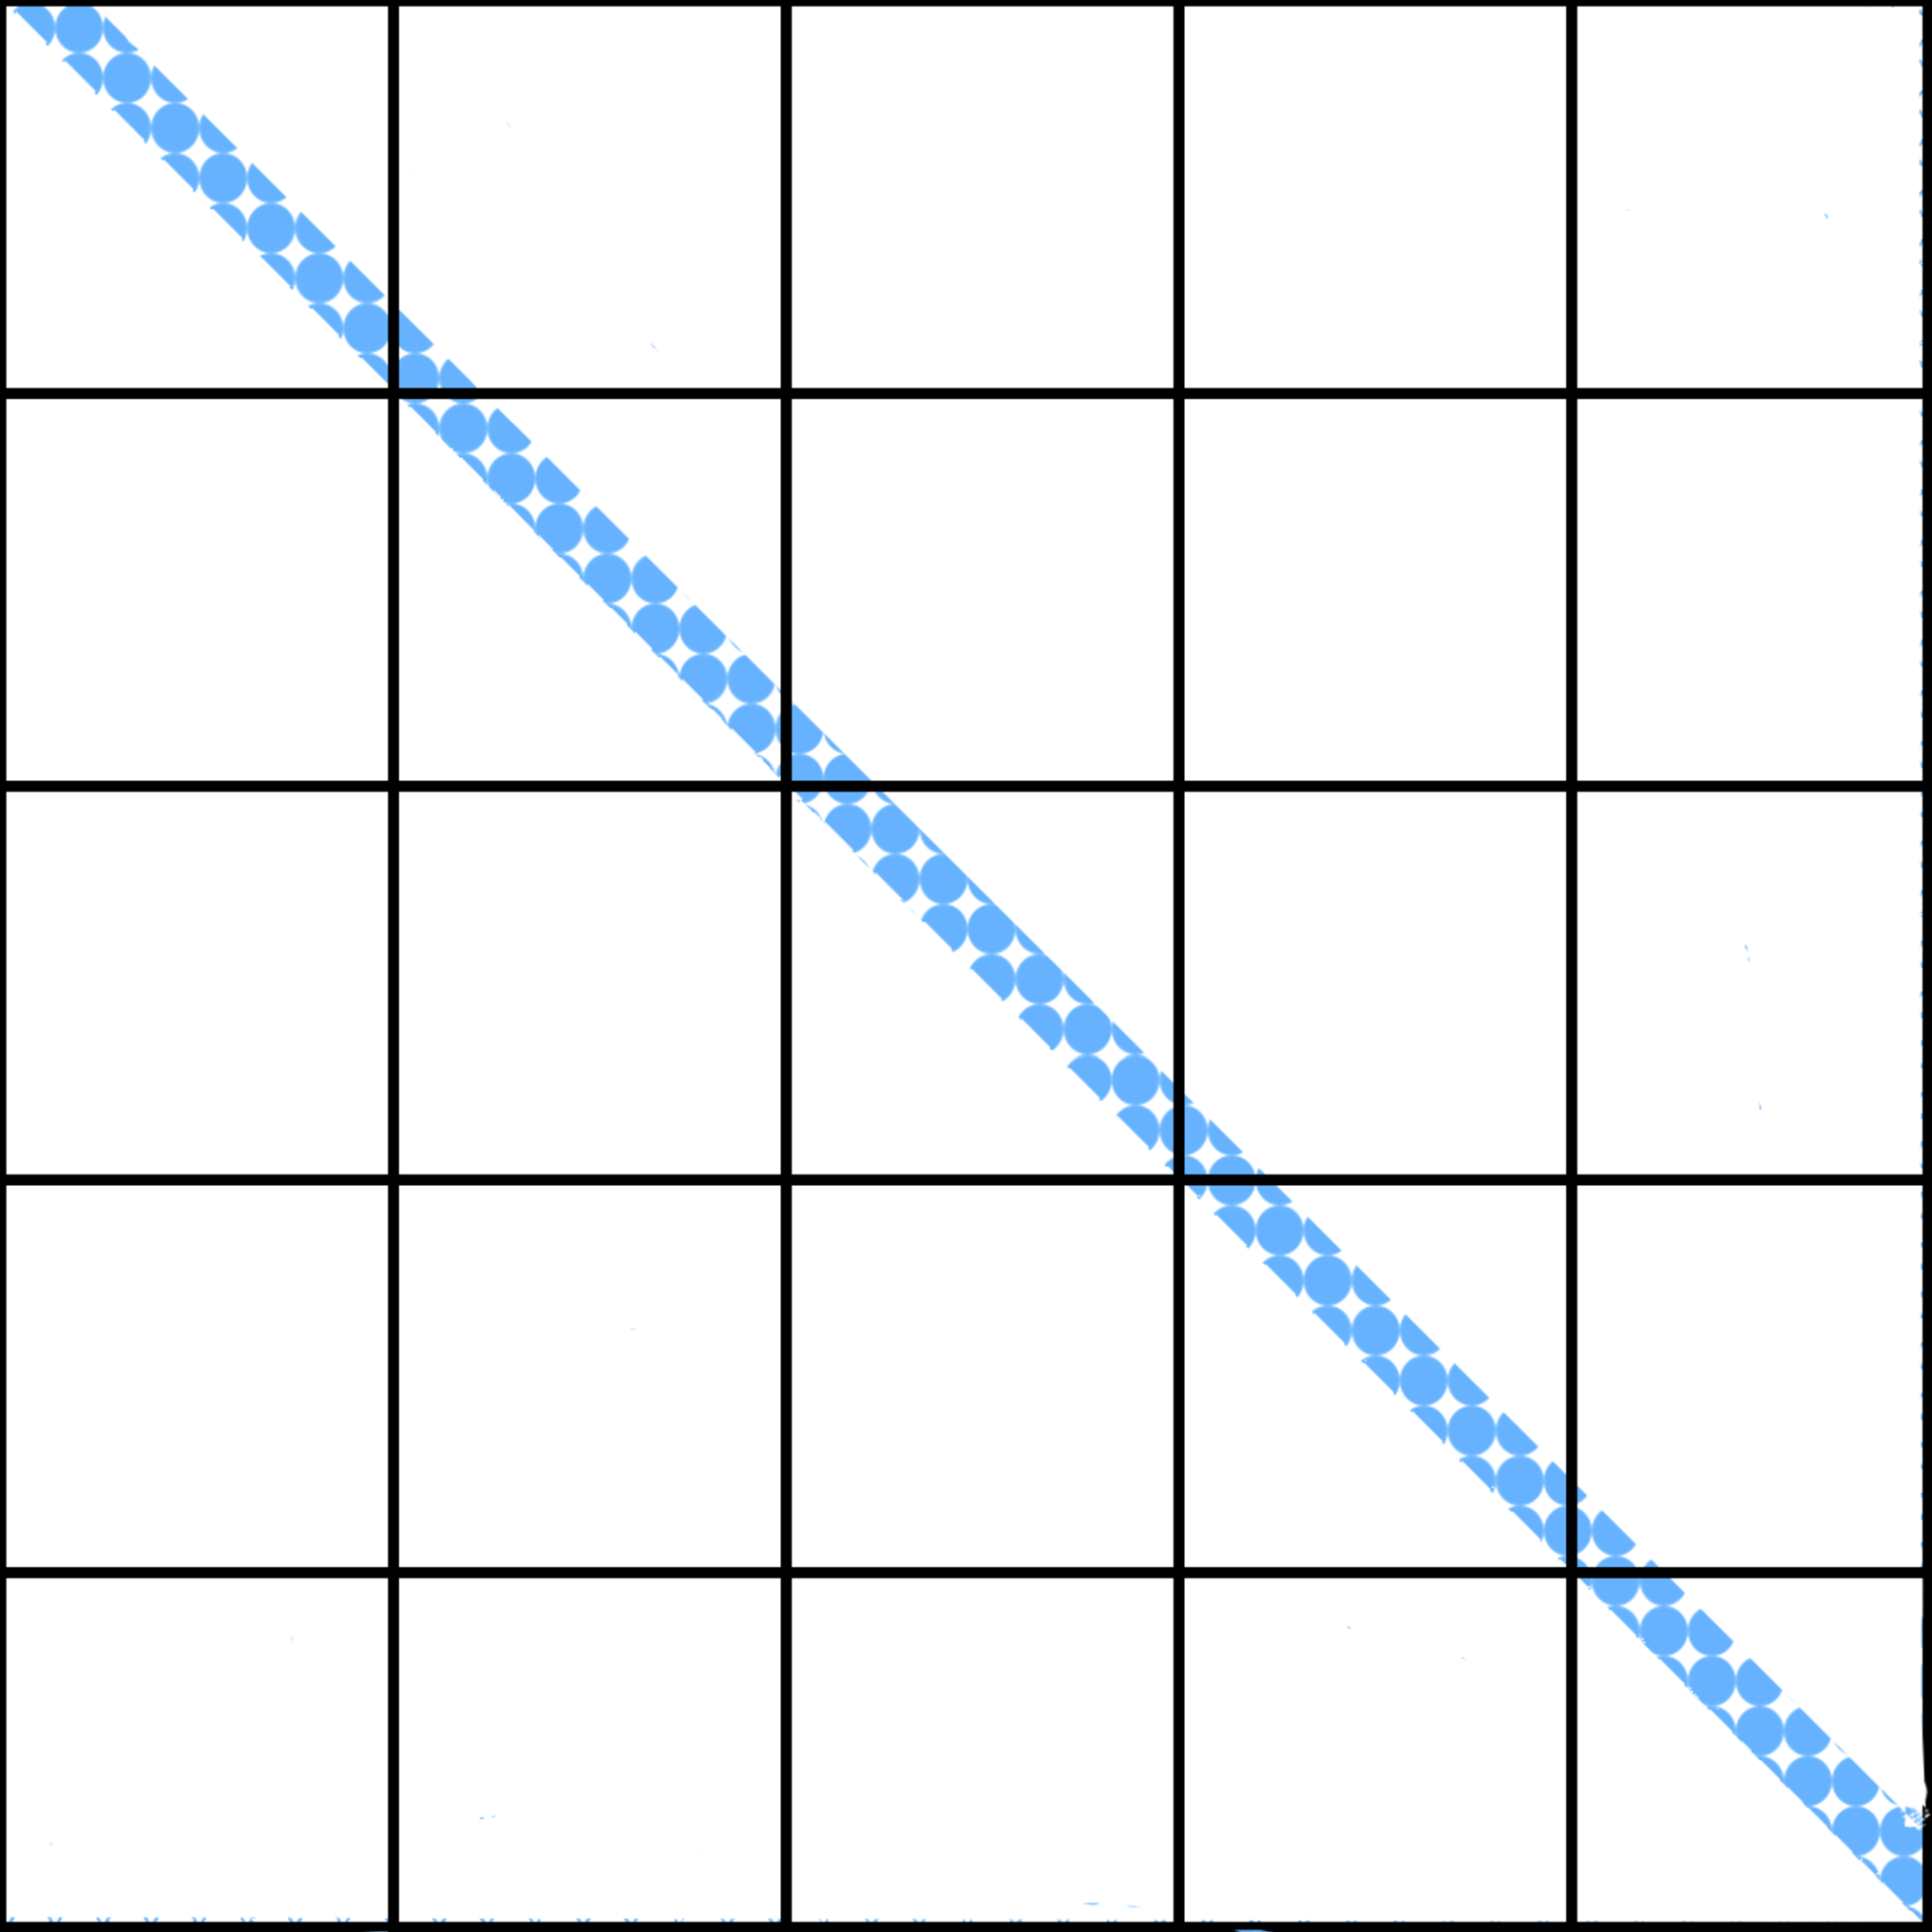
\includegraphics[width=3.5cm, height=3.5cm]{fig/SVD_bidiag}
    \caption{\label{fig:SVD_bidiag}
     Bidiagonal form.}
    \end{subfigure}
    \caption{Illustration of the two-stage bidiagonal reduction process.}
    \label{fig:two_stage}
\end{figure}
